%% ============================================================================
\documentclass[12pt,dvipdfmx]{jarticle}
\usepackage[hiresbb]{graphicx}
\usepackage[dvipdfmx,hidelinks]{hyperref}
\usepackage{multirow}
\usepackage{bigstrut}


%% ----------------------------------------------------------------------------
%% ページレイアウト設定
%% ----------------------------------------------------------------------------
\setlength{\textwidth}{40zw} %行の長さを全角40文字に設定(→ p280)
\setlength{\topmargin}{-0.51cm}
\setlength{\textheight}{23.7cm}

\setlength{\oddsidemargin}{-0.04cm} % 左マージンの設定
\renewcommand{\baselinestretch}{1.35}
% \pagestyle{empty} % すべてのページ番号を消去
%% ----------------------------------------------------------------------------

%% ----------------------------------------------------------------------------
%% 参考文献の設定
%% ----------------------------------------------------------------------------
% \usepackage[longnamesfirst]{natbib}
% \renewcommand{\bibname}{参考文献}
%% ----------------------------------------------------------------------------

\title{知能システム論 中間レポート}



%% ============================================================================

\begin{document}
% \maketitle
{\LARGE 知能システム論 中間レポート}
\begin{flushright}

\end{flushright}

\vspace{12pt}
第2回講義:探索に基づく問題解決 (1)の研究課題02-02について報告する.
\vspace{-0.5cm}
\paragraph*{研究課題02-02}
図02-02-01に示すグラフを深さ優先探索および幅優先探索で探索し, 探索過程におけるn,OpenList, ClosedListの変化を示せ. 初期状態はAとする.

\vspace{-1cm}
%% ----------------------------------------------------------------------------
\section*{1.木構造における探索手法}
%% ----------------------------------------------------------------------------

木構造における探索手法として,
ここでは深さ優先探索と幅優先探索を取り上げる.

どちらも,系統的探索による手法である.
系統的探索とは,順にしらみつぶし的に探索を行っていく方法である.

深さ優先探索とは,木構造において縦方向に探索を行う(図\ref{fig:01}).
一方の幅優先探索は図\ref{fig:02}に示すように,横方向の探索を行う.
% 深さ優先探索と幅優先探索の検索イメージを示す
\begin{figure}[h]
	\begin{minipage}{0.5\textwidth}
		\centering
		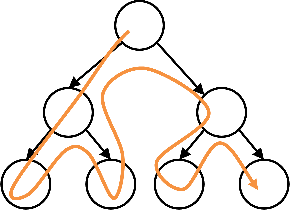
\includegraphics{fig01.png}
			\caption{深さ優先探索}
			\label{fig:01}
	\end{minipage}
	\begin{minipage}{0.5\textwidth}
		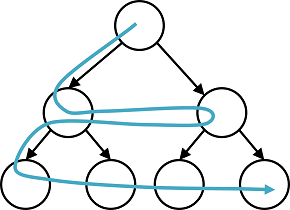
\includegraphics{fig02.png}
		\caption{幅優先探索}
		\label{fig:02}
	\end{minipage}
\end{figure}
\vspace{-1cm}
\subsection*{系統的探索の特徴}
汎用的な探索手法であり,理論的に解の発見が保証されるが,
計算量が大きいのが課題である.
探索対象となるデータの規模が大きいほど現実的な時間に収束しない恐れがある.
\vspace{-1cm}
\subsection*{木構造における他の探索手法}
それ以外の探索手法として,二分探索木 \cite{二分木} がある.

二分木は,子の数が最大2個までという制限を持たせた木構造である.
さらに各ノードの値よりも左の子ノードの方が値が小さくなる制約を持たせることで,
効率的な検索が可能となっている.

%二分探索木の例を掲載する

\vspace{-1cm}
%% ----------------------------------------------------------------------------
\section*{2.深さ優先探索と幅優先探索の探索過程の比較}
%% ----------------------------------------------------------------------------
図\ref{fig:02}に示すグラフを深さ優先探索および幅優先探索で探索し、探索過程におけるn,OpenList, ClosedListの変化を比較する。
\begin{figure}[h]
	\centering
	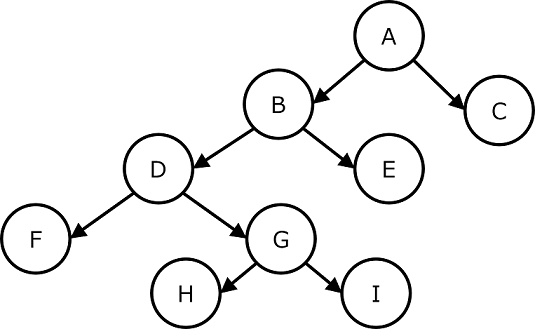
\includegraphics{fig03.png}
	\caption{比較に用いたグラフ}
	\label{fig:03}
\end{figure}

\vspace{-1cm}
\subsection*{実装したプログラムについて}
探索プログラムはpythonで実装を行った.
pythonは木構造を表現できるライブラリとしてanytree\cite{Anytree}があるが,
深さ優先探索および幅優先探索の実装や探索過程の表示には適さないため,anytreeは採用せずに2次元配列を用いた.

プログラムのソースコードは,本レポートとは別に添付する.

%\vspace{-1cm}
\subsection*{プログラムにおける木構造の表現}
作成したプログラムにおける木構造のデータ構造を表\ref{table:01}に示す.
今回取り上げるグラフは子が2個以下であるため,二分木のデータ構造とした.

	\begin{table}
		\centering
		\caption{図3のデータ構造}
		\label{table:01}
		\begin{tabular}{|c|c|c|c|}
		\hline
		Index & Node & 子ノード(左) &子ノード(右)  \\ \hline
		0 & A & 1 & 2 \\
		1 & B & 3 & 4 \\
		2 & C & 0 & 0 \\
		3 & D & 5 & 6 \\
		4 & E & 0 & 0 \\
		5 & F & 0 & 0 \\
		6 & G & 7 & 8 \\
		7 & H & 0 & 0 \\
		8 & I & 0 & 0 \\
		\hline
		\end{tabular}
	\end{table}


\subsection*{ 探索過程の比較結果}
初期状態とAとし,深さ優先探索および幅優先探索の過程を比較した.
目標をEとした場合のそれぞれの結果を表\ref{table:02}~\ref{table:03}に示す.

\begin{table}
	\begin{minipage}{0.5\textwidth}
		\centering
		\caption{深さ優先探索の探索過程}
		\label{table:02}
		\begin{tabular}{|c|c|c|}
			\hline
			n & OpenList &  CloseList \\ \hline
 			& A &  \\ \hline
			A &  & A \\ \hline
			A & BC & A \\ \hline
			B & C & BA \\ \hline
			B & DEC & BA \\ \hline
			D & EC & DBA \\ \hline
			D & FGEC & DBA \\ \hline
			F & GEC & FDBA \\ \hline
			G & EC & GFDBA \\ \hline
			G & HIEC & HGFDBA \\ \hline
			H & IEC & IHGFDBA \\ \hline
			I & EC & EIHGFDBA \\ \hline
			E & C & EIHGFDBA \\ \hline
 		\end{tabular}
	\end{minipage}
	\begin{minipage}{0.5\textwidth}
		\centering
		\caption{幅優先探索の探索過程}
		\label{table:03}
		\begin{tabular}{|c|c|c|}
			\hline
			 n & OpenList &  CloseList \\ \hline
			 & A &  \\ \hline
			A &  & A \\ \hline
			A & BC & A \\ \hline
			B & C & BA \\ \hline
			B & CDE & BA \\ \hline
			C & DE & CBA \\ \hline
			D & E & DCBA \\ \hline
			D & EFG & DCBA \\ \hline
			E & FG & EDCBA \\ \hline
		\end{tabular}
	\end{minipage}
 \end{table}

\vspace{-1cm}
%% ----------------------------------------------------------------------------
\section*{3.考察}
%% ----------------------------------------------------------------------------
今回の例では,幅優先探索の方が早く目標Eの探索ができた.
しかしながら,深さ優先探索と幅優先探索のどちらが有効であるか単純比較することはできない.
探索対象の木構造(深い構造か,幅が広い構造か)や目標の位置(根に近いか,葉に近いか)によって,効率性が大きく変わるからである.

そのため,規模の大きい木構造で探索を行う場合,木全体を探索するのではなく,
部分木に分割して探索対象を限定して実施するのがよい.

今回は初期状態を根であるAとしたが,初期状態をA以外とした場合(例えばD),
上位のAやBは探索されずに終わってしまう.
その場合にも,「部分木に分割して部分木の根から探索を開始する,その結果見つからない場合は次の部分木について探索を行う」
とすることで,解決することができる.


%% ----------------------------------------------------------------------------
%% 参考文献の出力
%% ----------------------------------------------------------------------------

\begin{thebibliography}{1}

\bibitem{二分木}
二分木(バイナリツリー)とは - IT用語辞典 e-Words
\newblock https://e-words.jp/w/二分木.html
\bibitem{Anytree} Any Python Tree Data , https://anytree.readthedocs.io/en/latest/
\bibitem{深さ優先探索}深さ優先探索(Wikipedia)
	\newblock https://ja.wikipedia.org/wiki/深さ優先探索
\bibitem{幅優先探索}幅優先探索(Wikipedia)
	\newblock https://ja.wikipedia.org/wiki/幅優先探索

\end{thebibliography}

\end{document}